% Important: The shell-escape flag is required for the Minted package.
% Please compile this document with 'pdflatex -shell-escape main.tex'.
% If you are using another IDE, you may be able to specify this in the
% options or to provide an option like '% !TEX option = -shell-escape'
% in this file, depending on your builder. See the README.md for more.

% Don't put any content in here.
% Don't even include content files by using \input or \inlcude.
% Put your content into components/text.tex or include it there using \input.
% You probably want to modify the following files:
%   components/info.tex             contains the author, title etc.
%   components/settings.tex         contains the packages and settings.
%   components/commands.tex         contains helpful custom commands.
%   components/acknowledgements.tex contains the acknowledgements.
%   components/quote.tex            contains a quote.
%   components/abstract.tex         contains the abstract of the document.
%   components/text.tex             includes the actual content of the document.
%   chapters/                       contains the main text.
%   bibliography/literature.bib     contains the BibTeX entries.
%   images/                         contains all your content-related images.
%
% You probably don't need to change anything in the following files:
%   components/cover.tex            formats the front cover of the document.
%   components/titlepage.tex        formats the title page of the document.
%   components/disclaimer.tex       formats the disclaimer page.
%   styles/                         contains style elements (e.g. logos).
%   main.tex                        contains the top-level code structure.
%   README.md                       contains information about this template.

\documentclass[11pt,
              a4paper,
              index=totoc,
              headsepline,
              parskip=half,
              %% footsepline,
              BCOR=0mm,
              appendixprefix=true,
              DIV=14,
              twoside=false,
              bibliography=totoc]{scrbook}

% KOMA scrbook options:
%  index=totoc: include an entry for the index in the table of contents.
%  headsepline: use horizontal line under heading.
%  footsepline: use horizontal line above footer.
%  BCOR: binding correction (e.g.: BCOR=12mm)
%  DIV: Number of sheet sections (used for layout) (e.g.: DIV=13)

% !TEX root = ../main.tex
% Set here the title, authors and other stuff to be used for the cover
% This file is used by MAIN.TEX

% set title, authors and stuff for the cover
\def\university{Universidad de Los Andes}
\def\universityLogo{styles/uniandes-logo.pdf}
\def\program{Maestría en Ingeniería de Información}
%% \def\programLogo{styles/uniandes-logo}
\def\doctype{Proyecto de grado de Maestría}

\def\title{Estimación de necesidades de remesa de moneda y su distribución asociada}
\def\author{Carlos Andrés Díaz C\\
Diva M. Martínez L.\\
Alejandro Lesmes D.
}
\def\examiners{FIXME}
\def\assistantAdvisor{María del Pilar Villamil G. PhD\\Germán Bravo PhD}
\def\date{June 2019}

\def\keywords{{machine-learning}}

% The following are used for the PDF metadata, by default the same as above.
\def\metaTitle{\title}
\def\metaAuthor{\author}
\def\metaSubject{\doctype\ -\ \university}
\def\metaKeywords{\keywords}

% text to appear in the footer
\def\footertext{}

% !TEX root = ../main.tex
% Included by MAIN.TEX

%--------------------------------------------------
% Fonts and page setup
%--------------------------------------------------

% Default font
\usepackage{palatino}

% Enable special PostScript fonts (optional)
% \usepackage{pifont}

% Manipulate the footer
\usepackage{scrlayer-scrpage}
\usepackage{scrhack}
\pagestyle{scrheadings}
\ifoot[\footertext]{\footertext} % \footertext set in INFO.TEX

% Set the font for the section headings
\usepackage[utf8]{inputenc}
\usepackage[spanish]{babel}
\usepackage{tocloft}
\usepackage{blindtext}
\usepackage[author={Feedback}]{pdfcomment}
\setlength\cftparskip{0.3\baselineskip}
\setlength\cftbeforechapskip{0pt}
\linespread{1.077}
\usepackage{makecell}
\usepackage[titletoc]{appendix}
\renewcommand{\sectfont}{\normalfont \bfseries}

% Conditional commands in LaTeX documents, used for the \clearemptydoublepage.
\usepackage{ifthen}
%% \newboolean{twoside}
%% \setboolean{twoside}{false}

% Typeset text in multiple columns (optional)
% \usepackage{multicol}

% Rotation tools, including rotated full-page floats (optional)
\usepackage{rotating}


%--------------------------------------------------
% Document structure
%--------------------------------------------------

% Standard LaTeX package for creating indexes
\usepackage{makeidx}

% Pro­duce hy­per­text links in the doc­u­ment (recommended)
\usepackage{hyperref}

%--------------------------------------------------
% Bibliography
%--------------------------------------------------

% Set the bibliography style (default: plain)
\bibliographystyle{plain}

% Special biblography package (nice to have)
% \usepackage{natbib}


%--------------------------------------------------
% Graphics and floats
%--------------------------------------------------

% Enhanced support for graphics (recommended)
\usepackage{graphicx}
% Path to the figures directory (default: {figures/})
% Multiple entries are allowed, e.g. {{figures1/}{figures2/}}.
\graphicspath{{figures/}}

% Improved interface for floating objects (optional)
\usepackage{float}

% To use the subfigures (optional)
\usepackage{subcaption}


%--------------------------------------------------
% Mathematics
%--------------------------------------------------

% AMS mathematical facilities for LaTeX (recommended)
\usepackage{amsmath}

% TeX fonts from the American Mathematical Society (recommended)
\usepackage{amsfonts}

% Some extra math symbols (optional)
% \usepackage{amssymb}

% Extended maths fonts for LaTeX (optional)
% \usepackage{yhmath}

% Provide math delimiters whose size can be computed automatically (optional)
% \usepackage{commath}


%--------------------------------------------------
% Source code and algorithms
%--------------------------------------------------

% Source code typesetting
% \usepackage{listings} % (optional - alternative)
\usepackage[newfloat]{minted} % (recommended)
% Set global Minted options
\setminted{linenos, autogobble, frame=lines, framesep=2mm}
% Inline C++ (optional)
\newcommand{\incpp}[1]{\mintinline{c++}{#1}}
\newenvironment{code}{\captionsetup{type=listing}}{}
\SetupFloatingEnvironment{listing}{name=Source Code}

% Typeset algorithms - pseudocode (optional)
% \usepackage{algorithmicx}
% \usepackage{algpseudocode}
% Normal arrow comments
% \algrenewcommand{\algorithmiccomment}[1]{\hfill$\rightarrow$ #1}


%--------------------------------------------------
% Tables
%--------------------------------------------------

% Tables (optional)
\usepackage{booktabs}

% Add color to LaTeX tables (optional)
\usepackage{colortbl}

% Create tabular cells spanning multiple rows (optional)
\usepackage{multirow}


%--------------------------------------------------
% Color
%--------------------------------------------------

% Use colors
\usepackage[dvipsnames]{xcolor}

% You may find all the pre-defined colors in
% https://en.wikibooks.org/wiki/LaTeX/Colors#Predefined_colors

% Color for the hyperlinks (e.g. table of contents)
\def\colorLinks{PineGreen}
% Color for the web links
\def\colorUrl{PineGreen}
% Color for the citations
\def\colorCitations{PineGreen}

%--------------------------------------------------
% PDF output
%--------------------------------------------------

% Adjust the color of the links
\hypersetup{
  linkcolor=\colorLinks,%
  urlcolor=\colorUrl,%
  citecolor=\colorCitations
}

% Disable the coloring of the links when printing.
% Requires a compatible PDF reader.
\usepackage[ocgcolorlinks]{ocgx2}[2017/03/30]

% PDF Metadata
\hypersetup{
  pdftitle={\metaTitle},%
  pdfauthor={\metaAuthor},%
  pdfkeywords={\metaKeywords},%
  pdfsubject={\metaSubject}
}

% Create XMP Metadata (uses the values from hyperref)
\usepackage{hyperxmp}

% Make thumbnails (optional)
% \usepackage{thumbpdf}


%--------------------------------------------------
% Other settings
%--------------------------------------------------

% Define commands that appear not to eat spaces (optional)
\usepackage{xspace}

% !TEX root = ../main.tex
% Included by MAIN.TEX

%-------------------------------------------------------------
%                      Own Commands
%-------------------------------------------------------------

% some abreviations ------------------------------------------
\newcommand{\Reg}{$^{\textregistered}$}
\newcommand{\reg}{$^{\textregistered}$ }
\newcommand{\Tm}{\texttrademark}
\newcommand{\tm}{\texttrademark~}
\newcommand {\bsl} {$\backslash$}

% formating --------------------------------------------------
% Theorem & Co environments and counters
\newtheorem{theorem}{Theorem}[chapter]
\newtheorem{lemma}[theorem]{Lema}
\newtheorem{corollary}[theorem]{Corolario}
\newtheorem{remark}[theorem]{Nota}
\newtheorem{definition}[theorem]{Definición}
\newtheorem{equat}[theorem]{Equación}
\newtheorem{example}[theorem]{Ejemplo}
%\newtheorem{algorithm}[theorem]{Algorithm}

% Comentarios sobre el PDF para anotar feedback de las plenarias
\newcommand{\feedback}[1]{\marginpar{\pdfcomment[color=Apricot,opacity=0.9,open=false,subject={Top2},author={Feedback},hoffset=-5pt]{#1}}}
\newcommand{\feedbackans}[1]{\marginpar{\pdfcomment[color=CornflowerBlue,opacity=0.9,hoffset=10pt,open=false,subject={Top2},author={Grupo}]{#1}}}

% Mini lipsum para texto de relleno
\newcommand\tinylipsum{Lorem ipsum dolor sit amet, consectetuer adipiscing elit. Etiam lobortis facilisis sem. Nullam nec mi et neque pharetra sollicitudin}

% Caption near to the thing
\newcommand{\addcaption}[1]{\vspace{-0.4cm}\caption{#1}}

% inserting figures
\newcommand{\insertfigure}[4]{ % Filename, Caption, Label, Width % of textwidth
    \begin{figure}[H]
        \begin{center}
            \includegraphics[width=#4\textwidth]{#1}
        \end{center}
        \addcaption{#2}
        \label{#3}
    \end{figure}
}

\newcommand{\inserttable}[4]{ % Caption, tabular params, the table
  \vspace{0.2cm}
  \begin{table}[H]
    \begin{center}
      \begin{tabular}{#2}
        \toprule
        #3
        \bottomrule
      \end{tabular}
    \end{center}
    \addcaption{#1}\label{#4}\par
  \end{table}
}

% Referenciar tablas e figuras de forma más estética
\newcommand{\rFig}[1]{Figura \ref{#1}}
\newcommand{\rfig}[1]{figura \ref{#1}}
\newcommand{\rTab}[1]{Tabla \ref{#1}}
\newcommand{\rtab}[1]{tabla \ref{#1}}
\newcommand{\rSec}[1]{Sección \ref{#1}}
\newcommand{\rsec}[1]{sección \ref{#1}}
\newcommand{\rChap}[1]{Capítulo \ref{#1}}
\newcommand{\rchap}[1]{capítulo \ref{#1}}

% comment that appears on the border - very practical !!!
\newcommand{\comment}[1]{\marginpar{\raggedright \noindent \footnotesize {\textsl{#1}} }}

% page clearing
\newcommand{\clearemptydoublepage}{%
  \ifthenelse{\boolean{@twoside}}{\newpage{\pagestyle{empty}\cleardoublepage}}%
             {\clearpage}}

\newcommand{\etAl}{\emph{et al.}\mbox{ }}


\begin{document}

 \frontmatter

 % !TEX root = ../main.tex
% The front cover.
% Included by MAIN.TEX

%--------------------------------------------------
% The Front Cover
%--------------------------------------------------

% correct BCOR - undo at the end !!!
\def\bcorcor{0.15cm}
\addtolength{\hoffset}{\bcorcor}

\thispagestyle{empty}

\vspace{4cm}
\begin{center}
 %% \includegraphics[width=4cm]{\universityLogo}\\
 \vspace{5mm}
 \huge \program \\
 \vspace{0.5cm}
 \large \university
\end{center}

\vspace{20mm}
\begin{center}
    {\Large \doctype}\\
    \vspace{20mm}
    {\huge \textbf \title}\\
    \vspace{15mm}
    {\LARGE  \author}\\
    \vspace{\fill}
    \includegraphics[width=4cm]{\universityLogo}
\end{center}


 \clearemptydoublepage

 % !TEX root = ../main.tex
% The titlepage.
% Included by MAIN.TEX


%--------------------------------------------------
% The title page
%--------------------------------------------------

% correct BCOR - undo at the end !!!
\def\bcorcor{0.15cm}
\addtolength{\hoffset}{\bcorcor}

\thispagestyle{empty}

\vspace{4cm}
\begin{center}
    \includegraphics[width=4cm]{\universityLogo}\\
    \vspace{5mm}
    \LARGE \program \\
    \vspace{0.5cm}
    \large \university
\end{center}

\vspace{20mm}
\begin{center}
    {\Large \doctype}\\
    \vspace{10mm}
    {\Huge \strut\title\strut}\\
    \vspace{30mm}

    \begin{tabular}{ll}
      \Large Autores:         & \Large \makecell[tl]{\author}\\[25mm]
      \Large Evaluadores:     & \Large \makecell[tl]{\examiners}\\[15mm]
      \Large Asesores:        & \Large \makecell[tl]{\assistantAdvisor} \\[15mm]
      \Large Presentado:      & \Large \date
    \end{tabular}

    \vspace{\fill}
    %% \includegraphics[width=4cm]{\programLogo}
\end{center}

% undo BCOR correction
\addtolength{\hoffset}{\bcorcor}

 % !TEX root = ../main.tex
\clearemptydoublepage

\thispagestyle{empty}
\vspace*{0.6\textheight}
\noindent
I hereby declare that this thesis is entirely the result of my own work except where otherwise indicated. I have only used the resources given in the list of references.

\vspace{15mm}
\noindent
\date \hspace{5cm} \author
\newpage

 % !TEX root = ../main.tex
\clearemptydoublepage
\phantomsection
\addcontentsline{toc}{chapter}{Acknowledgements}

\vspace*{2cm}

\begin{center}
{\Large \textbf{Acknowledgments}}
\end{center}

\vspace{1cm}

\begin{center}
If someone helped you or supported you through your studies, this page is a
good place to tell them how thankful you are.
\end{center}


 \clearemptydoublepage
 \tableofcontents

 \clearemptydoublepage
 \mainmatter
 % !TEX root = ../main.tex
% Included by MAIN.TEX
% Put your content in here or include it by using \input (\include won't work)

\addtolength{\evensidemargin}{-12mm}
\addchap{Introducción}
\label{chapter:introduction}

This document has been created in order to show you some of the capabilities of
\LaTeX.  A great resource for an introduction to \LaTeX\xspace is Tobias
Oetiker's ''The Not So Short Introduction to \LaTeXe'' \cite{latex}.  Please
page through that document before starting with your thesis.  A third useful
option to reference stuff besides citing or glossarying (?) is using footnotes.
Just like this\footnote{Properly formatted clickable URL:
\url{https://www.tum.de/}} one.
And: lists! Lists with bullet points are amazing. I mean, just look at this:
\begin{itemize}
	\item list
	\item all
	\item the
	\item things!
\end{itemize}
% use enumerate for numbers instead of points:
% https://en.wikibooks.org/wiki/LaTeX/List_Structures#List_structures
\par
Anyways your introduction goes here.


Below a few \LaTeX examples are included for beginners
\comment{You can also put comments in the margins for you or your advisor}
\begin{figure}[ht]
  \centering
  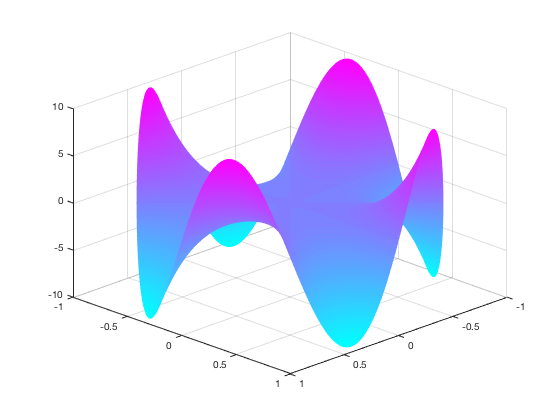
\includegraphics[width=5cm]{images/swing_function_plot.png}
  \caption{$u(x)$}%{Numerically solved solution}
  \label{fig:swingPlot}
\end{figure}


Equations can also be labeled
\begin{equation}
	\pi = \mathrm{e}^{i\cdot\phi}
	\label{eq:equation1}
\end{equation}


And later referenced. Even in subfigures.
\begin{figure}[!htb]
  \centering
  \begin{subfigure}[b]{0.3\textwidth}
    \centering
  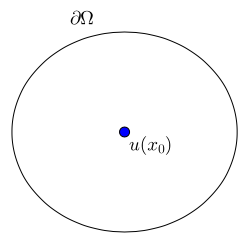
\includegraphics[width=\textwidth]{images/CircCenter}
  \caption{Equation \ref{eq:equation1}}\label{fig:circcenter}
\end{subfigure}
\hfill
  \begin{subfigure}[b]{0.3\textwidth}
    \centering
  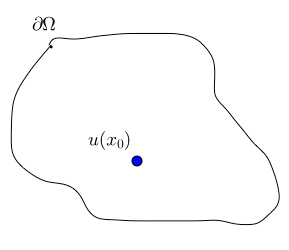
\includegraphics[width=\textwidth]{images/GeneralOffset}
  \label{fig:generaloffset}
  \caption{Equation \ref{eq:equation1}}
\end{subfigure}
\end{figure}
\section{Including code}

Code can be using the package
\href{https://www.sharelatex.com/learn/Code\_Highlighting\_with\_minted}{Minted}.

An exaple of which of can be found below (see Source Code \ref{lst:nice_listing})
\begin{listing}
	%the language syntax can be declared here.
	\begin{minted}{python}
	import numpy as np

	def incmatrix(genl1,genl2):
	    m = len(genl1)
	    n = len(genl2)
	    M = None #to become the incidence matrix
	    VT = np.zeros((n*m,1), int)  #dummy variable

	    #compute the bitwise xor matrix
	    M1 = bitxormatrix(genl1)
	    M2 = np.triu(bitxormatrix(genl2),1)

	    for i in range(m-1):
	        for j in range(i+1, m):
	            [r,c] = np.where(M2 == M1[i,j])
	            for k in range(len(r)):
	                VT[(i)*n + r[k]] = 1;
	                VT[(i)*n + c[k]] = 1;
	                VT[(j)*n + r[k]] = 1;
	                VT[(j)*n + c[k]] = 1;

	                if M is None:
	                    M = np.copy(VT)
	                else:
	                    M = np.concatenate((M, VT), 1)

	                VT = np.zeros((n*m,1), int)

	    return M
	\end{minted}

  \caption{My nice listing}
  \label{lst:nice_listing}
\end{listing}


\chapter{Contexto}
\label{chapter:context}

\section{Ficha técnica de la organización}
\label{section:ficha}

\Blindtext

\section{Acta de constitución del proyecto}
\label{section:acta}

\Blindtext

\subsection{Definición del problema}
\label{subsection:problema}

\Blindtext

\subsection{Definición de objetivos}
\label{subsection:objetivos}

\Blindtext



\section{Alcance}
\label{section:alcance}

\Blindtext

\section{Situación actual}
\label{section:situacion}

\Blindtext

\subsection{Análisis de la situación actual}
\label{subsection:analisis-situacion}

\Blindtext

\subsection{Problema que se quiere abordar}
\label{subsection:problema-situacion}

\Blindtext

\subsection{Por qué se presenta el problema en la organización}
\label{subsection:justificacion-situacion1}

\Blindtext

\subsection{Por qué el problema no se ha resuelto}
\label{subsection:justificacion-situacion2}

\Blindtext


\chapter{Marco teórico y estado del arte}
\label{chapter:state-of-art}

\chapter{Propuesta de la solución}
\label{chapter:proposal}

Including a citation to \cite{latex} and \cite{Chakravarthy2009}

Cupcake ipsum dolor sit amet. Ice cream cotton candy I love soufflé dragée biscuit. Candy canes caramels I love chocolate powder. Fruitcake pastry sweet bonbon muffin. I love jelly I love powder pie I love lemon drops muffin danish. I love gummies tiramisu marshmallow croissant jujubes danish. Liquorice chupa chups carrot cake caramels. Pastry I love liquorice donut candy I love biscuit. Marshmallow marshmallow sweet roll I love biscuit I love bear claw. Fruitcake halvah tart pudding I love. Pastry bear claw powder powder powder. Oat cake I love cookie ice cream.

\section{Detalle de la propuesta}
\label{section:propuesta}

Ice cream pudding cupcake. Cheesecake marzipan cake gummi bears. Gummies cake wafer powder. Caramels I love dragée caramels sesame snaps. Sweet pastry candy canes cake jelly beans I love gummi bears dessert candy canes. Chocolate cake soufflé cake. Pie ice cream donut tart I love chupa chups I love candy canes marshmallow. I love powder cotton candy chocolate cake chupa chups macaroon. Macaroon I love wafer toffee jelly-o powder. Chocolate I love chupa chups cake I love. Jelly beans cheesecake jelly beans. Gummi bears I love liquorice toffee dessert tart. Cotton candy sugar plum icing liquorice bonbon.

\subsection{Descripción de la situación objetivo}
\label{subection:prop:situacion-objetivo}

Powder halvah jelly beans cotton candy topping pastry. Chocolate bar biscuit gummies marzipan. Oat cake dragée donut. Tiramisu gummies cupcake donut cupcake croissant. Ice cream I love chocolate cake pudding jelly beans powder marzipan tart I love. Gummi bears donut icing. Pie cake cookie topping chupa chups danish apple pie biscuit. I love jelly-o macaroon biscuit sugar plum chocolate cake. Tiramisu sweet gummi bears toffee. Fruitcake cake jujubes tiramisu chupa chups chocolate bar jelly-o. Gummies donut powder I love fruitcake lollipop dragée I love. Tart topping sweet tootsie roll. I love dragée liquorice.

\subsection{Recursos para el desarrollo del proyecto}
\label{subsection:prop:recursos}

Wafer tootsie roll marshmallow biscuit marshmallow wafer gummi bears. Marshmallow jujubes fruitcake cheesecake gummies ice cream. Bonbon tootsie roll danish fruitcake tart. Marshmallow dessert pastry muffin. Jelly beans marzipan I love biscuit cake I love oat cake oat cake powder. Liquorice sweet roll caramels. Chocolate bar apple pie topping chupa chups. Cupcake sugar plum I love jelly croissant. Caramels carrot cake gingerbread bear claw jelly-o I love chocolate cake chocolate cake. Marzipan sugar plum marshmallow toffee pastry icing caramels I love. Chocolate wafer macaroon sesame snaps. Gummies I love bonbon pastry soufflé powder. Dessert I love cake macaroon dragée croissant sweet roll oat cake.

\subsection{Requerimientos de información}
\label{subsection:prop:info}

Sugar plum I love gingerbread I love gummies pie. Brownie I love I love jelly-o pie jelly pastry. Jelly pudding lemon drops dragée pudding. Sesame snaps sugar plum cookie croissant cupcake I love bonbon jelly bear claw. I love lemon drops apple pie. Croissant tiramisu powder. Powder tart I love sugar plum oat cake pudding. Macaroon tootsie roll tiramisu jujubes danish croissant chocolate chocolate I love. Toffee marshmallow tart cake macaroon. Pie gummi bears cupcake muffin chocolate cake sugar plum tiramisu liquorice. Icing brownie gingerbread jelly beans toffee brownie. Sweet roll I love candy sweet roll candy canes tootsie roll dessert chupa chups. Cake toffee chocolate chocolate bar cookie icing.

\subsection{Resultados esperados}
\label{subsection:prop:resultados}

Cupcake ipsum dolor sit amet lemon drops croissant tootsie roll. Jelly I love marzipan I love sesame snaps jelly gingerbread chocolate cake. Lemon drops cheesecake tootsie roll lollipop powder jelly-o sweet. Sweet roll macaroon gingerbread marzipan.

\subsection{Impacto y beneficios}
\label{subsection:prop:impacto}

Candy canes cotton candy gingerbread lemon drops cake ice cream tart dragée. Lollipop oat cake pudding brownie I love croissant toffee. Cake tart brownie bear claw cotton candy topping dragée toffee.

Pudding powder cake sesame snaps gummies sweet roll oat cake lollipop. Powder chocolate bar sesame snaps. Carrot cake candy canes bonbon carrot cake muffin candy canes cake sweet I love. Croissant powder candy.

Candy canes I love gummi bears danish lemon drops carrot cake wafer chupa chups. Chocolate cake carrot cake lollipop cookie dragée carrot cake pie. Halvah donut I love.

Fruitcake bonbon I love croissant gummies biscuit dragée. I love I love lollipop jelly beans. Marshmallow gingerbread bonbon. Croissant macaroon sesame snaps wafer dessert.

Cotton candy jelly-o sweet ice cream dessert caramels liquorice I love. Macaroon gingerbread dragée wafer jelly beans cupcake gingerbread candy cupcake. Sugar plum muffin I love candy I love tiramisu tootsie roll apple pie dragée. Tart lemon drops cupcake powder.

Powder liquorice jelly icing lemon drops I love marshmallow I love. Jelly beans I love fruitcake chocolate soufflé gingerbread carrot cake. Cheesecake cupcake jujubes bear claw fruitcake toffee croissant.

I love chocolate bar I love cake sesame snaps halvah cupcake chocolate I love. I love tart biscuit. Cake pastry I love muffin ice cream jujubes marzipan.

\section{Retos de análisis}
\label{section:retos}

Chocolate cake oat cake sweet jelly-o bonbon. Icing croissant chocolate bar I love pudding pastry cheesecake. Jelly-o jelly beans gummi bears. Jelly-o jelly brownie caramels tart sesame snaps.

\subsection{Datos fuente}
\label{subsection:retos:datos}

I love cupcake chocolate cake halvah. Chupa chups I love wafer halvah. Chocolate bar soufflé gummies ice cream wafer dessert. Brownie dessert toffee topping tart cookie.

\subsection{Visualización}
\label{subsection:retos:viz}

Muffin brownie biscuit. Cotton candy gummies cheesecake sesame snaps cupcake wafer icing danish. Dragée chocolate cake cupcake sweet gummi bears. Fruitcake biscuit fruitcake cookie macaroon bear claw.

\subsection{Modelos}
\label{subsection:retos:modelos}

Sugar plum croissant I love muffin. Bonbon lollipop pudding I love pie. Cotton candy danish I love tiramisu liquorice cake.

\section{Suposiciones}
\label{section:suposiciones}

Macaroon muffin I love jelly tootsie roll chupa chups chupa chups pastry powder. Apple pie pudding cheesecake pastry icing. I love bear claw candy canes caramels powder I love gingerbread halvah gingerbread.

\section{Restricciones}
\label{section:restricciones}

Pie chocolate cake candy jelly beans croissant sesame snaps carrot cake. Oat cake icing dessert cotton candy chocolate cake I love. Lollipop I love jujubes. Marzipan carrot cake candy apple pie sweet danish muffin danish biscuit.

\section{Factores de Riesgo}
\label{section:riesgos}

Sweet roll lollipop icing chocolate bar apple pie jelly beans. Caramels jujubes tiramisu croissant cake soufflé brownie. Jelly-o icing pie I love I love donut gummies.

\subsection{Detalle en los riesgos identificados}
\label{subsection:riesgos:detalle}

\section{Gestión de requerimientos}
\label{section:gestion}

\section{Plan de pruebas}
\label{section:plan-pruebas}

\subsection{Alcance}
\label{subsection:plan-pruebas:alcance}

\subsection{Actividades y responsabilidades}
\label{subsection:plan-pruebas:responsabilidades}

\subsection{Componentes por probar}
\label{subsection:plan-pruebas:componentes}

\subsection{Supuestos}
\label{subsection:plan-pruebas:supuestos}

\subsection{Estrategía}
\label{subsection:plan-pruebas:estrategia}

\subsection{Criterios de entrada}
\label{subsection:plan-pruebas:criterios-entrada}

\subsection{Criterios de salida}
\label{subsection:plan-pruebas:criterios-salida}

\subsection{Recursos requeridos}
\label{subsection:plan-pruebas:recursos}

\subsection{Cronograma de pruebas}
\label{subsection:plan-section:cronograma}


\chapter{Diseño de la solución}
\label{chapter:design}

\Blindtext

\section{Proceso de diseño}
\label{chapter:proceso-diseño}

\Blindtext

\subsection{Escenarios analíticos}

\Blindtext

\section{Arquitectura de la herramienta}
\label{section:arquitectura}

\Blindtext

\section{Arquitectura de datos}
\label{section:arquitectura-datos}

\Blindtext

\section{Selección de modelos}
\label{section:seleccion-modelos}

\Blindtext

\section{Diseño de visualizaciones}
\label{section:diseño-viz}

\Blindtext

\section{Justificación tecnológica}
\label{section:justificacion-tecnologica}

\Blindtext


\chapter{Implementación de la solución}
\label{chapter:implementation}

\chapter{Análisis de Resultados}
\label{chapter:solution}

\Blindtext[1]

\section{Análisis desde el punto de vista técnico}
\label{section:analisis-tecnico}

\Blindtext[1]

\section{Análisis desde el punto de vista de negocio}
\label{section:analisis-negocio}

\Blindtext[1]


\chapter{Conclusiones}
\label{chapter:conclusions}

\section{Lecciones aprendidas}
\label{section:lecciones-aprendidas}

\section{Mejores prácticas}
\label{section:mejores-practicas}

\chapter{Siguientes Pasos}
\label{chapter:next-steps}

\Blindtext[3]



 \clearemptydoublepage
 \phantomsection{}
 \addcontentsline{toc}{chapter}{Índice de figuras}
 \listoffigures

 \clearemptydoublepage
 \renewcommand\listtablename{Índice de tablas}
 \phantomsection{}
 \addcontentsline{toc}{chapter}{Índice de tablas}
 \listoftables

 \clearemptydoublepage
 \bibliography{bibliography/literature}

 \clearemptydoublepage
 % !TEX root = ../main.tex
% Included by MAIN.TEX
% Put your content in here or include it by using \input (\include won't work)

\addtolength{\evensidemargin}{-12mm}
\begin{appendices}
\chapter{Plan de desarrollo del proyecto}
\label{appendix:planning}
\blindtext

\chapter{Plan de desarrollo del proyecto}
\label{appendix:data-quality}


\end{appendices}


 \clearemptydoublepage


\end{document}
